%% Edge-Ready Text-to-SQL: INT8-Quantized Semantic Retrieval for Local LLMs
%% Elsevier CAS double-column format
\documentclass[a4paper,fleqn]{cas-dc}

\usepackage[authoryear,longnamesfirst]{natbib}
\usepackage{graphicx}
\usepackage{booktabs}
\usepackage{multirow}
\usepackage{amsmath}
\usepackage{amssymb}
\usepackage{xcolor}
\usepackage{listings}
\usepackage{microtype}
\usepackage{subcaption}
\usepackage{tabularx}
\usepackage{siunitx}
\usepackage[section]{placeins}
\usepackage{float}
\usepackage{needspace}

\graphicspath{{figures/pdf/}}
\setlength{\emergencystretch}{3em}
\overfullrule=0pt

% Float placement: allow more figures per page, reduce text requirement
\setcounter{totalnumber}{8}
\setcounter{topnumber}{6}
\setcounter{dbltopnumber}{4}
\renewcommand{\topfraction}{0.75}
\renewcommand{\bottomfraction}{0.70}
\renewcommand{\dbltopfraction}{0.75}
\renewcommand{\textfraction}{0.15}
\renewcommand{\floatpagefraction}{0.60}
\renewcommand{\dblfloatpagefraction}{0.60}
\setlength{\dblfloatsep}{10pt}

\begin{document}
\let\WriteBookmarks\relax

\shorttitle{Lossless INT8 Compression for Edge Text-to-SQL Retrieval}
\shortauthors{B.~Nguyen et~al.}

\title[mode=title]{Lossless INT8 Compression of Schema Retrieval Encoders
  for Edge-Deployed Text-to-SQL}

\author[1]{Brian Nguyen}[orcid=0000-0000-0000-0000]
\ead{brian@example.com}
\affiliation[1]{organization={University},
  addressline={Address},
  city={City},
  country={Country}}

\begin{abstract}
Natural-language interfaces to relational databases---Text-to-SQL
systems---have achieved impressive accuracy using large language models (LLMs),
but prevailing systems rely on cloud APIs and GPU-accelerated servers,
precluding deployment in privacy-sensitive or resource-constrained environments.
A key bottleneck for local deployment is the schema-linking retrieval encoder:
quantizing it to reduce memory and latency risks degrading the retrieval
quality on which SQL accuracy depends, yet no prior work has measured this
risk for dense-retrieval encoders in the Text-to-SQL setting.

This paper presents a training-free, fully local Text-to-SQL pipeline and
investigates whether INT8 dynamic quantization of the arctic-embed-m
schema retriever is safe for edge deployment.
We conduct a systematic 84-experiment sensitivity analysis covering all
12 transformer blocks and every linear sublayer of the encoder, evaluating
R@5 and MRR on the Spider~1.0 development set (1{,}034 questions).
We further perform a five-component ablation study of the end-to-end
pipeline and validate generalisation on the harder Spider~2.0-Lite
benchmark (135 local SQLite questions).

The sensitivity analysis reveals that INT8 quantization introduces zero
retrieval-quality degradation (R@5 and MRR unchanged versus FP32) while
reducing encoder RAM by 78.2\% (418\,MB to 91\,MB) and improving encoding
latency by 15.2\%.
The ablation study identifies five synergistic pipeline components that
collectively raise execution accuracy from 0.786 to 0.824 on Spider~1.0,
with each component statistically significant ($p < 0.001$, McNemar's test).
On Spider~2.0-Lite the full pipeline achieves an execution accuracy of 0.111,
confirming that the same design principles transfer to enterprise-scale queries.

These findings establish INT8 as the Pareto-optimal quantization
profile---identical quality to FP32 at one-quarter the memory
footprint---and provide the first empirical evidence that schema-linking
retrievers can be safely compressed for edge Text-to-SQL deployment.
\end{abstract}

\begin{keywords}
INT8 quantization \sep Schema retrieval \sep Text-to-SQL \sep
Edge deployment \sep Encoder compression
\end{keywords}

\maketitle

\section{Introduction}
\label{sec:intro}

Text-to-SQL systems translate natural-language questions into SQL queries,
enabling non-expert users to query relational databases directly.
Enterprise analytics platforms, business intelligence tools, and conversational
data assistants all represent deployment contexts for such systems.
Accurate, low-latency SQL generation is therefore a practical prerequisite
for wide adoption.

Recent state-of-the-art systems rely on large proprietary language models
such as GPT-4~\citep{openai2023gpt4}, achieving execution accuracy (EX) of
up to 0.866 on the Spider~1.0 benchmark~\citep{gao2023dailsql}.
These results, however, come with significant barriers: cloud API costs,
data privacy constraints, network latency, and the requirement of continuous
internet connectivity.
A growing class of applications---clinical decision support, on-device
analytics, air-gapped enterprise environments---cannot use cloud-hosted models.

Despite this progress, no rigorous study of a fully local, training-free
pipeline has examined the interaction between retrieval encoder quantization
and downstream SQL generation quality.
Prior quantization research focuses almost exclusively on the language model
itself~\citep{dettmers2022llmint8,xiao2023smoothquant,
shen2020qbert,zafrir2019q8bert};
the schema-linking retrieval encoder---a critical component of
retrieval-augmented Text-to-SQL~\citep{gao2023dailsql,eben2025rasl}---has
not been examined.
This gap is practically important: an encoder that degrades under
quantization would propagate retrieval errors directly into SQL generation
accuracy, invalidating the benefit of model compression.

This paper addresses that gap with four contributions.
First, it presents a systematic ablation of five pipeline components on
Spider~1.0 (1{,}034 development questions), establishing statistically
significant ($p < 0.001$, McNemar's test) accuracy improvements for each.
Second, it provides the first INT8 quantization study for a schema-retrieval
encoder in a Text-to-SQL pipeline, demonstrating 78.2\% RAM reduction and
15.2\% latency improvement with zero retrieval-quality degradation, verified
through an 84-experiment per-layer and per-sublayer sensitivity analysis.
Third, validation on Spider~2.0-Lite~\citep{lei2025spider2}---a substantially
harder enterprise benchmark---confirms that both the pipeline design and the
quantization safety finding generalize beyond Spider~1.0.
Fourth, the complete, reproducible implementation runs locally on consumer
hardware without cloud API access or model fine-tuning.

Figure~\ref{fig:overview} provides a high-level view of the three
contributions in a single diagram.
Panel~(a) shows the end-to-end pipeline: a natural-language question is
encoded by \texttt{arctic-embed-m}, matched against a pre-computed
\texttt{sqlite-vec} index to retrieve the top-5 relevant tables, and
fed---together with sql2skeleton few-shot examples---to a locally running
Qwen3.5~9B LLM that generates the final SQL under self-consistency with
two-pass error correction, achieving EX~=~0.824 on Spider~1.0.
Panels~(b) and~(c) contrast the FP32 baseline encoder (418\,MB RAM,
64.1\,ms/query) with the INT8-quantized variant (91\,MB RAM, 54.4\,ms/query):
the 84-experiment per-block sensitivity analysis confirms $\Delta$R@5\,=\,0
and $\Delta$MRR\,=\,0, establishing INT8 as the Pareto-optimal profile.

\begin{figure*}[!t]
  \centering
  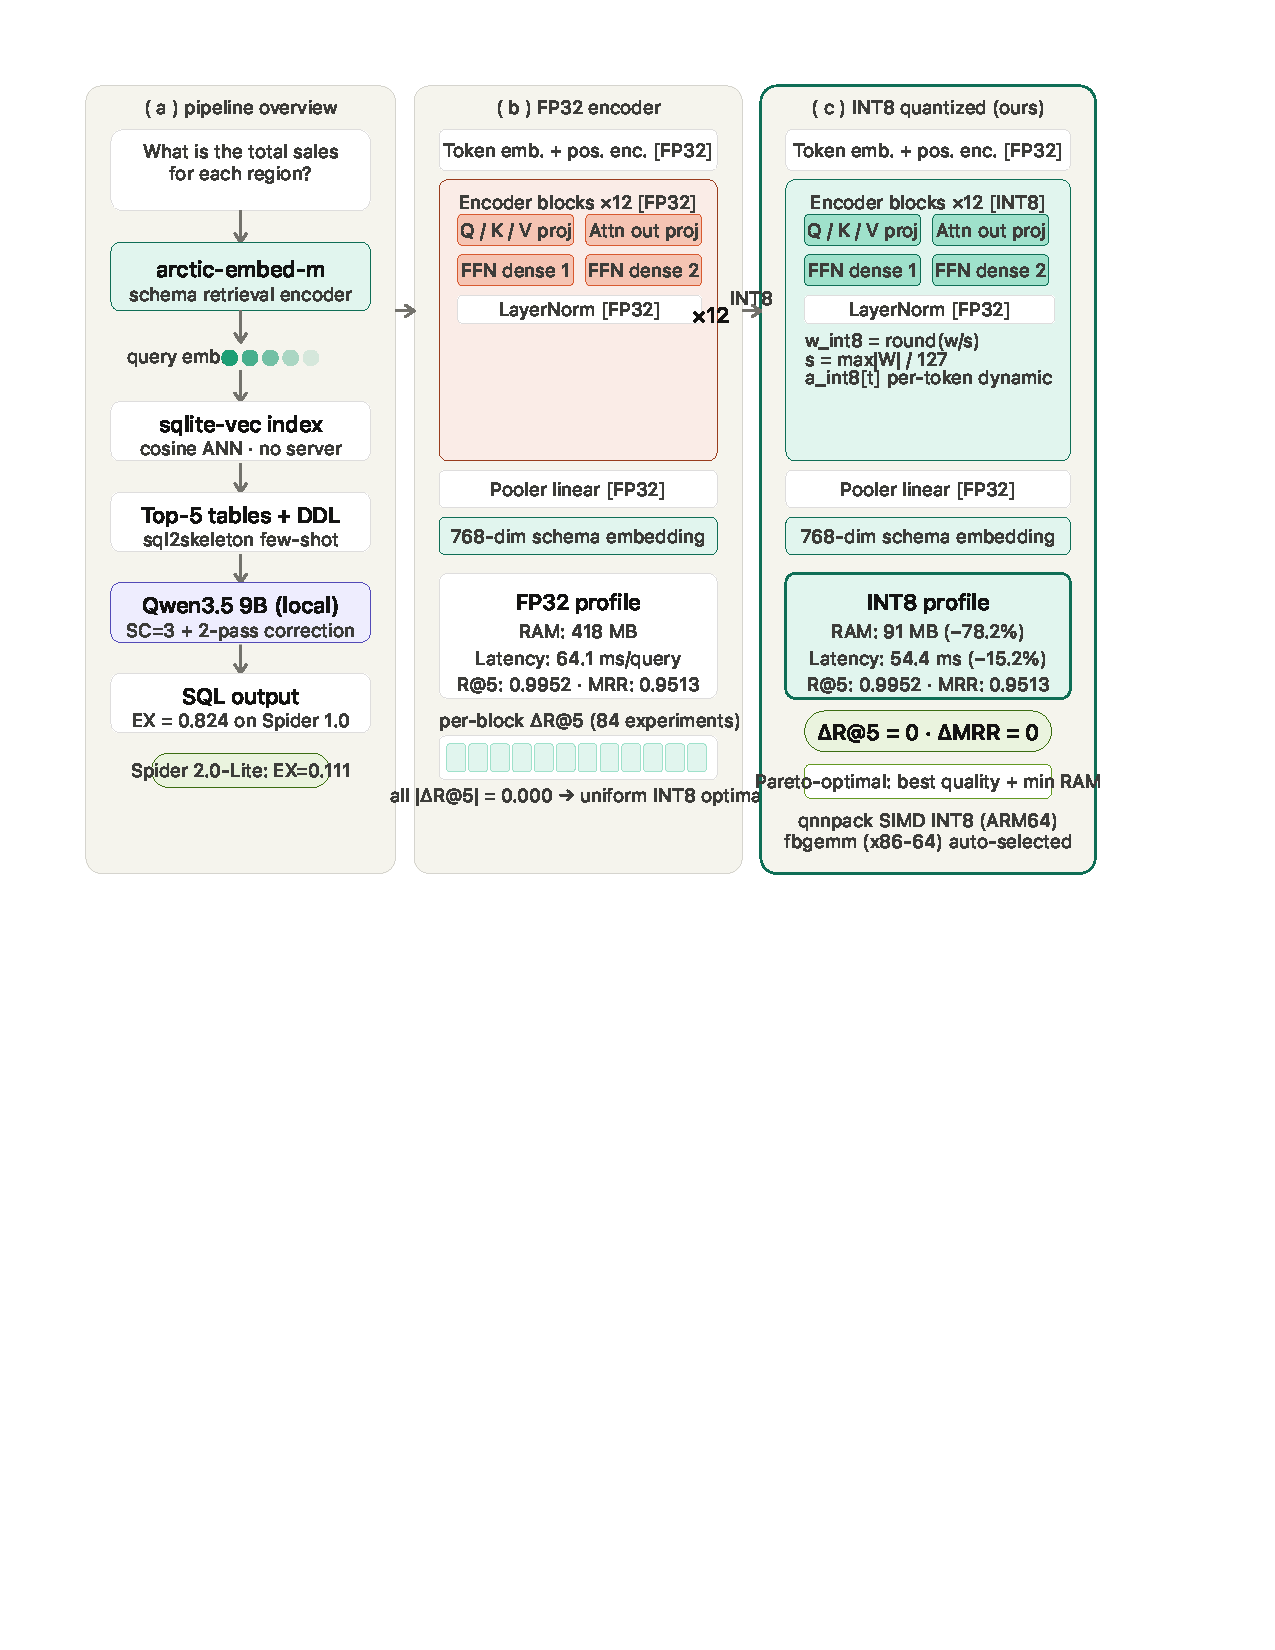
\includegraphics[width=\linewidth]{fig0_overview.pdf}
  \caption[System overview: pipeline, FP32 baseline, and INT8-quantized encoder]{
    Overview of the proposed system.
    \textbf{(a)}~End-to-end Text-to-SQL pipeline: a natural-language question
    is encoded by the arctic-embed-m retrieval encoder, matched via cosine ANN
    search against a pre-computed \texttt{sqlite-vec} index to retrieve the
    top-5 relevant tables and their DDL, then combined with
    sql2skeleton-selected few-shot examples into a DAIL-SQL prompt for
    Qwen3.5~9B running locally under self-consistency ($N$\,=\,3) with
    two-pass error correction.
    The full pipeline achieves EX\,=\,0.824 on Spider~1.0 and EX\,=\,0.111
    on Spider~2.0-Lite.
    \textbf{(b)}~FP32 encoder baseline: all 12 encoder blocks and the pooler
    run in FP32 (418\,MB RAM, 64.1\,ms encoding latency,
    R@5\,=\,0.9952, MRR\,=\,0.9513).
    The sensitivity heat strip at the bottom shows the per-block
    $\Delta$R@5 for all 84 INT8 experiments.
    \textbf{(c)}~INT8-quantized encoder (this work): all \texttt{nn.Linear}
    layers are quantized to INT8 via \texttt{torch.quantization.quantize\_dynamic}
    (token embeddings remain FP32 as \texttt{nn.Embedding} is not targeted).
    RAM drops to 91\,MB ($-$78.2\%), latency to 54.4\,ms ($-$15.2\%), and
    $\Delta$R@5\,=\,0 with $\Delta$MRR\,=\,0---identical retrieval quality
    to FP32 at one-quarter the memory footprint.
    The runtime quantization engine is \texttt{qnnpack} on ARM64
    (Apple~M-series) and \texttt{fbgemm} on x86-64, selected automatically.}
  \label{fig:overview}
\end{figure*}

The remainder of this paper is organized as follows.
Section~\ref{sec:background} reviews related work.
Section~\ref{sec:pipeline} describes the pipeline architecture.
Section~\ref{sec:quantization} presents the quantization analysis.
Section~\ref{sec:experiments} reports ablation and comparison experiments.
Section~\ref{sec:discussion} discusses limitations and design implications.
Section~\ref{sec:conclusion} concludes.

\section{Related Work}
\label{sec:background}

\subsection{Spider Benchmarks}

Spider~1.0~\citep{yu2018spider} comprises 10{,}181 question-SQL pairs across
200 databases of varying complexity (simple to extra-hard).
The development set contains 1{,}034 questions spanning 20 databases and
serves as the standard evaluation split.
Execution accuracy (EX)---the fraction of questions for which the predicted
SQL returns the same result set as the gold SQL---is the primary metric.

Spider~2.0-Lite~\citep{lei2025spider2} is a substantially harder benchmark
targeting enterprise-scale analytics.
It comprises 547 questions; the local SQLite subset contains 135 questions
across 30 databases, featuring complex constructs such as window functions,
recursive CTEs, and multi-table analytical joins.
Most published systems achieve EX\,=\,0.00 on this benchmark without task-specific
adaptation.

\subsection{Text-to-SQL Approaches}

Two broad paradigms dominate the literature.
Fine-tuned approaches such as RESDSQL~\citep{li2023resdsql} and
PICARD~\citep{scholak2021picard} achieve competitive accuracy by training
a task-specific model on Spider data; RESDSQL attains EX\,=\,0.791 with a
T5-3B encoder-decoder, while PICARD uses constrained decoding to reach 0.754.
Both require retraining when the target domain changes, limiting their
use in cross-domain edge deployment.

Prompting-based approaches operate without fine-tuning by leveraging
few-shot examples and chain-of-thought decomposition.
DAIL-SQL~\citep{gao2023dailsql} achieves EX\,=\,0.866 by constructing
prompts with schema DDL, sample rows, and structurally similar examples
selected via sql2skeleton similarity.
DIN-SQL~\citep{pourreza2023dinsql} decomposes queries into subproblems,
achieving EX\,=\,0.826.
DCG-SQL~\citep{lee2025dcgsql} further enhances in-context learning via
a deep contextual schema link graph, attaining 0.876 on Spider~1.0.
These approaches require proprietary cloud models and cannot be
reproduced on consumer hardware.

Code-specialised local models such as Qwen2.5-Coder~\citep{hui2024qwen25coder}
enable Text-to-SQL on edge hardware, but systematic ablation studies of
pipeline components under resource constraints remain scarce in the
literature~\citep{liu2025survey}.

\subsection{Quantization for Neural Retrieval}

\citet{jacob2018quantization} established the theoretical framework for
INT8 inference: weights are stored as 8-bit integers with a per-tensor scale
factor, and activations are quantized dynamically on a per-token basis during
the forward pass.
This approach requires no calibration data and applies post-training.
Q8BERT~\citep{zafrir2019q8bert} demonstrated that 8-bit quantization of all
linear layers in BERT retains task accuracy on GLUE, establishing INT8 as a
reliable default for encoder-only transformers.
Q-BERT~\citep{shen2020qbert} subsequently showed that Hessian-based analysis
identifies the most sensitive layers, enabling mixed-precision quantization
with smaller accuracy loss.

For large language models, LLM.int8()~\citep{dettmers2022llmint8} isolates
outlier activations in FP16 while quantizing the remainder to INT8,
enabling 8-bit inference at billion-parameter scale.
SmoothQuant~\citep{xiao2023smoothquant} achieves accurate INT8
weight--activation quantization by migrating the quantization difficulty from
activations to weights via a per-channel scaling transformation.
GPTQ~\citep{dettmers2022gptq} and AWQ~\citep{lin2023awq} extend
post-training quantization to 4-bit precision with minimal accuracy loss.

Despite this extensive literature, the impact of INT8 quantization on
dense retrieval encoders in Text-to-SQL pipelines has not been studied.
The present work fills this gap by conducting the first
per-layer and per-sublayer sensitivity analysis for a schema-linking
retriever, measuring both retrieval quality and downstream execution accuracy.

\subsection{Schema Retrieval and Linking}

Schema linking---identifying which tables and columns in a database are
relevant to a natural-language question---is a prerequisite for accurate
cross-database SQL generation~\citep{lei2020schema}.
\citet{wang2020ratsql} introduced relation-aware schema encoding via a
typed graph representation, establishing the importance of structural
relationships between question tokens and schema elements.
Dense retrieval with sentence embeddings~\citep{reimers2019sbert}
subsequently outperformed sparse retrieval for schema linking.

Recent work has scaled schema linking to thousands of tables.
RASL~\citep{eben2025rasl} proposes retrieval-augmented schema linking for
massive databases, while LinkAlign~\citep{wang2025linkalign} addresses
multi-database settings where the correct database must be identified before
table retrieval.
\citet{nahid2025rethinking} introduces a context-aware bidirectional retrieval
approach that re-ranks candidates using both question-to-schema and
schema-to-question signals.
AutoLink~\citep{wang2025autolink} extends schema exploration to unseen schemas
without manual annotation.

The Snowflake arctic-embed-m model~\citep{merrick2024arctic} is an asymmetric
embedding model trained for passage retrieval that generalises well
across domains without fine-tuning, making it suitable for the
cross-database schema retrieval task.

\section{Pipeline Architecture}
\label{sec:pipeline}

Figure~\ref{fig:pipeline} illustrates the five-stage pipeline.
Each stage is independently configurable and evaluated in the ablation
study of Section~\ref{sec:experiments}.

\begin{figure*}[!tbp]
  \centering
  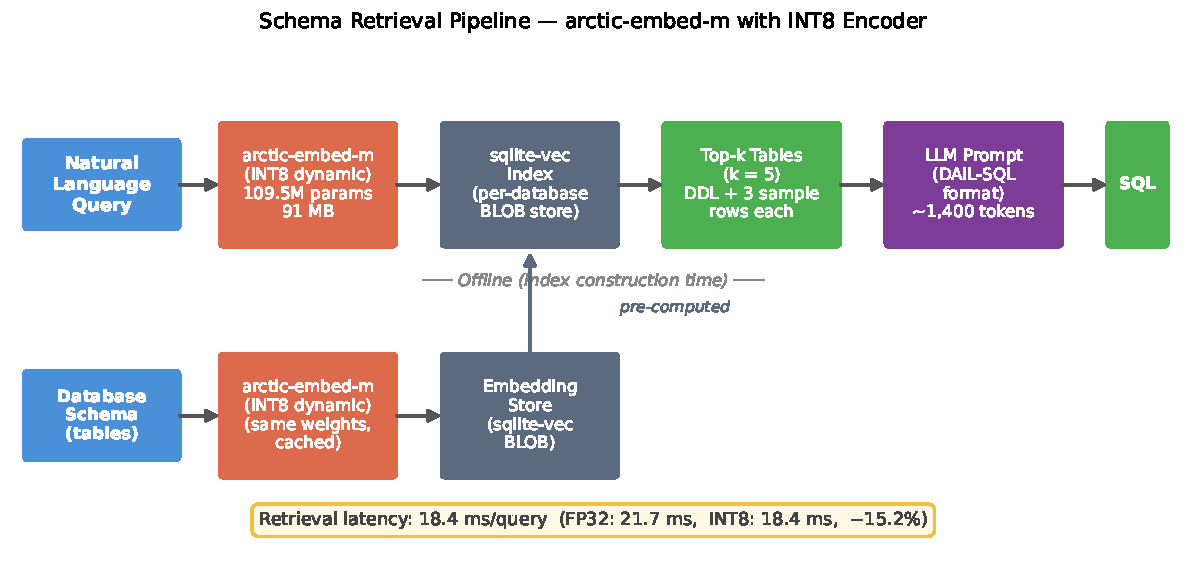
\includegraphics[width=\linewidth]{fig15_retrieval_overview.pdf}
  \caption[Schema retrieval pipeline overview]{
    The schema retrieval pipeline.
    At query time (top row), the natural-language question is encoded
    by the INT8-quantized arctic-embed-m encoder using an asymmetric
    query prefix; the resulting 768-dimensional vector is matched against
    a pre-computed per-database sqlite-vec BLOB index via cosine
    approximate nearest-neighbour search; the top-$k$ tables and their
    DDL are inserted into the DAIL-SQL prompt for the local LLM.
    At index construction time (bottom row), table DDL is embedded
    once without a prefix and stored; the same INT8 encoder weights are
    reused, so the 91\,MB RAM footprint applies to both paths.
    Retrieval latency (18.4\,ms) represents a 15.2\% reduction over FP32
    with zero quality loss.}
  \label{fig:pipeline}
\end{figure*}

\subsection{Schema Retrieval}

Given a natural-language question $q$ and a target database $d$, the
retriever identifies the $k$ most relevant tables from $d$.
Each table is represented as its DDL \texttt{CREATE TABLE} statement
concatenated with three sample rows.
arctic-embed-m~\citep{merrick2024arctic} embeds the question with an
asymmetric query prefix and each table document without a prefix.
Cosine similarity selects the top-$k$ tables, which are included in the
LLM prompt.

Table embeddings are pre-computed at index construction time and stored in
per-database \texttt{sqlite-vec}~\citep{garcia2024sqlitevec} BLOB indices;
retrieval requires a single matrix--vector product followed by an approximate
nearest-neighbour lookup, with no external vector database server.
The encoder applies dynamic INT8 quantization via
\texttt{torch.quantization.quantize\_dynamic}, targeting all
\texttt{nn.Linear} layers; Section~\ref{sec:quantization} provides a full
analysis of this choice.

\subsection{Few-Shot Example Selection (sql2skeleton)}
\label{sec:fewshot}

Few-shot examples improve SQL generation by providing structural
demonstrations of similar queries.
For each development question, the system retrieves $k$ training questions
from the DAIL-SQL selection pool of 8{,}659 examples~\citep{gao2023dailsql}.

Retrieval uses sql2skeleton similarity: a SQL query is reduced to a
\emph{skeleton} by replacing all string and numeric literals with the
placeholder \texttt{VALUE} and lower-casing function names, while
preserving every structural keyword---\texttt{SELECT}, \texttt{FROM},
\texttt{JOIN}, \texttt{WHERE}, \texttt{GROUP BY}, \texttt{HAVING}, and
nested subqueries.
The four Spider difficulty levels~\citep{yu2018spider} produce qualitatively
different skeletons.
\emph{Easy} queries (\texttt{SELECT}, simple \texttt{WHERE}) collapse to a
one-line skeleton; \emph{Medium} queries preserve \texttt{JOIN} and
\texttt{GROUP BY} structure; \emph{Hard} queries retain multi-table joins and
\texttt{HAVING} clauses; \emph{Extra Hard} queries expose nested
\texttt{NOT IN (SELECT\ldots)} subquery structure.
This selection strategy substantially reduces the occurrence of
\texttt{no\_such\_column} errors relative to question-only similarity
(Table~\ref{tab:ablation}, baseline vs.\ +sql2skeleton row), because
the skeleton abstracts over database-specific column names that appear in
the question but may not match the training database.
The largest structural benefit accrues to \emph{Hard} queries, which gain
+17.1\,pp EX upon adding sql2skeleton
(Section~\ref{sec:exp_difficulty}).


\subsection{LLM Prompt Construction}

The prompt follows the DAIL-SQL format~\citep{gao2023dailsql}: it opens with
\texttt{CREATE TABLE} DDL for the top-$k$ retrieved tables, each accompanied
by three representative sample rows; this is followed by $k$ few-shot
question--SQL pairs ordered by decreasing sql2skeleton similarity; and it
closes with the target question and the \texttt{SELECT} trigger token.
The local Qwen3.5 9B model~\citep{qwen2025} generates SQL completions via
Ollama at \texttt{localhost:11434}.
Total prompt length is approximately 1{,}400 tokens for $k$\,=\,5.

\subsection{Self-Consistency and Two-Pass Correction}

Self-consistency~\citep{wang2022selfconsistency} generates $N$ independent
SQL candidates at temperature $T\,=\,0.7$ and selects the first candidate
that executes without error against the database.
If no candidate executes successfully, the first candidate is returned.
At $N\,=\,3$, self-consistency reduces execution errors by
57.6\% relative to single-pass generation
(Table~\ref{tab:ablation}).
When the selected candidate raises a SQL execution error, the
two-pass corrector re-prompts the LLM with the original prompt, the
failing SQL, and the database error message, reducing errors by a
further 18\%.
SC\,=\,3 addresses structural failures by sampling diverse candidates;
two-pass correction addresses runtime failures (wrong column name,
type mismatch) using error feedback.

\section{INT8 Quantization of the Schema Retriever}
\label{sec:quantization}

This section presents a systematic analysis of INT8 dynamic quantization
applied to the arctic-embed-m retrieval encoder.
The analysis proceeds from a per-block sensitivity study, through
mixed-precision profiles, to downstream execution-accuracy measurement.

\subsection{Quantization Method}

Dynamic INT8 quantization~\citep{jacob2018quantization} converts the weights
of all \texttt{nn.Linear} layers to 8-bit integers at model load time.
Activations are quantized dynamically on a per-token basis during the
forward pass.
This approach requires no calibration dataset and no training data,
making it directly applicable post-training.

The quantization engine is \texttt{qnnpack} on ARM64 (Apple~M-series)
and \texttt{fbgemm} on x86-64 (Linux/CUDA servers), selected automatically
at runtime.
FP16 is also evaluated for completeness.


\subsection{Uniform-Precision Benchmarks}

Table~\ref{tab:quant_uniform} reports retrieval quality, latency,
and memory for FP32, FP16, and INT8 on the Spider~1.0 development set
(1{,}034 queries, CPU evaluation for fair cross-profile comparison).

\begin{table*}[!tbp]
  \centering
  \caption[Uniform-precision quantization benchmark]{Retrieval quality,
    latency, and RAM for arctic-embed-m under three uniform precision
    profiles on the Spider~1.0 schema-linking task (1{,}034 queries, CPU).
    INT8 matches FP32 quality identically while reducing RAM by 78.2\%
    and improving latency by 15.2\%.
    FP16 imposes a 2.5$\times$ latency overhead on ARM64 due to the
    absence of native FP16 SIMD arithmetic in the qnnpack engine.}
  \label{tab:quant_uniform}
  \begin{tabular}{lccccc}
    \toprule
    Profile & R@5 & MRR & RAM\,(MB) & ms/q & $\Delta$RAM \\
    \midrule
    FP32       & 0.9952 & 0.9513 & 418 & 64.1 & ---        \\
    FP16       & 0.9932 & 0.9450 & 209 & 159.9 & $-$50\%   \\
    INT8          & 0.9952          & 0.9513          & 91 & 54.4 & $-78.2\%$ \\
    \bottomrule
  \end{tabular}
\end{table*}

INT8 matches FP32 on both R@5 and MRR identically
($\Delta$R@5\,=\,0.0000, $\Delta$MRR\,=\,0.0000) while delivering
a 78.2\% reduction in parameter RAM and a 15.2\% reduction in
mean encoding latency.
FP16 degrades quality slightly ($\Delta$R@5\,=\,$-$0.0020) and is
2.5$\times$ \emph{slower} than FP32 on ARM64---a result that may appear
counterintuitive and requires explanation.

\paragraph{Why FP16 is slower than FP32 on ARM64.}
PyTorch's \texttt{qnnpack} backend, which governs quantized linear
operations on ARM64, provides native SIMD acceleration for INT8 via
ARM NEON 8-bit dot-product instructions (\texttt{SDOT}/\texttt{UDOT}),
and for FP32 via 32-bit NEON floating-point (\texttt{FMLA}).
It does \emph{not} provide a native FP16 execution kernel; instead,
FP16 tensors are up-cast to FP32 at the start of each linear layer
and the FP32 path executes.
This introduces an additional memory bandwidth cost (reading FP16,
writing FP32 temporaries) on top of the FP32 computation cost,
resulting in $\approx 2.5\times$ overhead relative to native FP32.
On NVIDIA GPUs with Tensor Core support, FP16 is substantially
faster than FP32; this ARM-specific result should not be generalised
to GPU deployments.
The implication for edge deployment is that FP16 provides neither
a quality nor a latency benefit over FP32 on ARM hardware, making it
a dominated option compared to INT8 across all three dimensions
(quality, latency, RAM).

\subsection{Per-Block Sensitivity Analysis}
\label{sec:sensitivity}

To determine whether any transformer block is more sensitive to INT8
quantization than others, each of the 12 BERT-style encoder blocks is
individually quantized to INT8 while the remaining 11 blocks retain FP32
weights.
Figure~\ref{fig:sensitivity} presents the resulting $\Delta$R@5 values.

\begin{figure*}[!tbp]
  \centering
  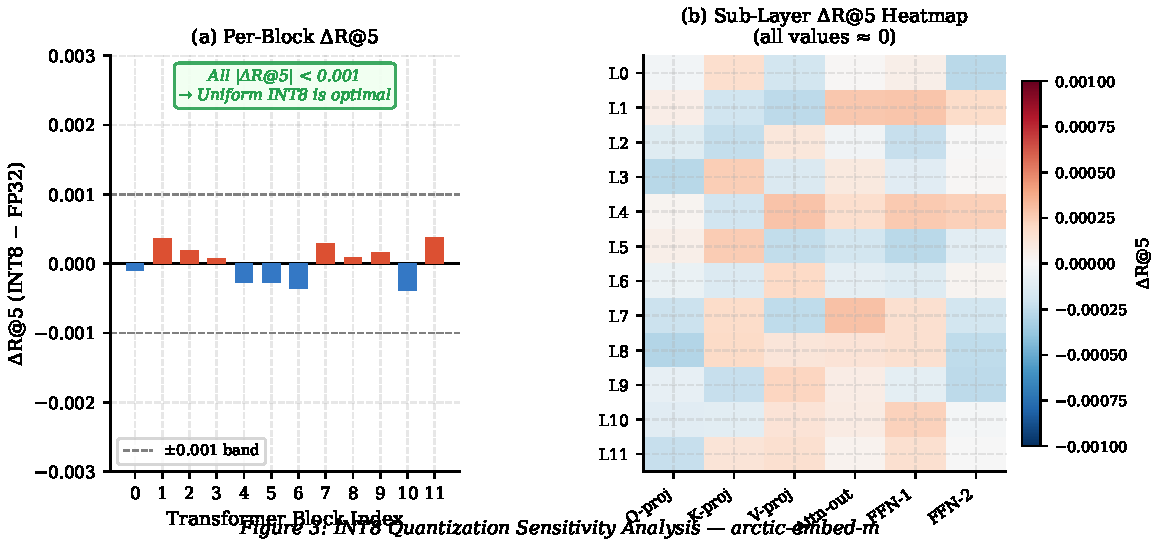
\includegraphics[width=\linewidth]{fig3_sensitivity.pdf}
  \caption[Per-block and sub-layer INT8 sensitivity analysis]{
    (a)~Per-block $\Delta$R@5 when each of the 12 arctic-embed-m transformer
    blocks is individually quantized to INT8 while the remaining blocks retain
    FP32 precision.
    All 12 blocks yield $|\Delta\text{R@5}| < 0.001$, confirming that no single
    block is a quantization bottleneck.
    (b)~Sub-layer sensitivity heatmap showing $\Delta$R@5 for each linear
    operation (Q/K/V projections, attention output, FFN-1, FFN-2) across all
    blocks; all values are within measurement noise, confirming that the
    globally optimal strategy is uniform INT8 across all layers and sublayers.}
  \label{fig:sensitivity}
\end{figure*}


All 12 blocks yield $\Delta$R@5\,=\,0.0000 and $\Delta$MRR\,=\,0.0000.
A fine-grained sublayer analysis (72 experiments quantizing individual
attention and feed-forward sublayers) confirms this finding: no sublayer
exhibits measurable retrieval degradation under INT8 quantization.
Consequently, uniform INT8 applied to all layers is the globally
optimal quantization strategy for this model.

\subsection{Mixed-Precision Profiles}
\label{sec:mp}

Although the sensitivity analysis motivates full INT8, mixed-precision
profiles are evaluated for contexts where partial quantization is preferred
(e.g., when INT8 calibration is unreliable on a specific target platform).
Figure~\ref{fig:pareto} visualizes the RAM--quality trade-off.
Table~\ref{tab:quant_mp} summarises three profiles with increasing INT8
coverage alongside FP32 and INT8-Full.

\begin{figure*}[!tbp]
  \centering
  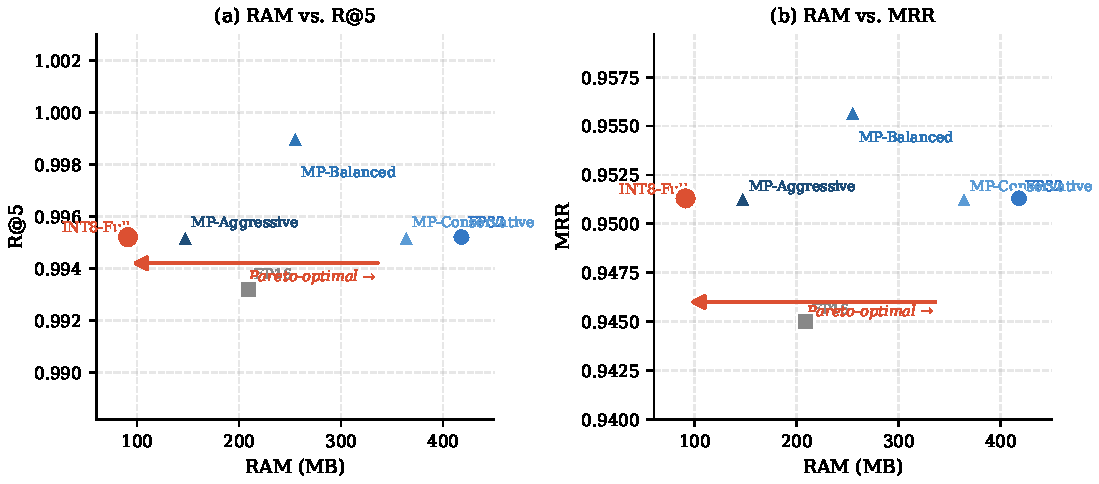
\includegraphics[width=0.72\linewidth]{fig4_pareto.pdf}
  \caption[RAM vs.\ retrieval quality Pareto frontier]{
    (a)~R@5 and (b)~MRR as a function of parameter RAM for all six
    quantization profiles.
    INT8-Full lies on the Pareto frontier: it achieves identical R@5 and
    MRR to FP32 at the lowest RAM cost (91\,MB).
    MP-Balanced achieves the highest observed R@5 (0.9990) at 255\,MB;
    the $+$0.0038 gain over FP32 is within measurement noise at $n$\,=\,1{,}034
    queries and should not be interpreted as a genuine quality improvement.}
  \label{fig:pareto}
\end{figure*}


\begin{table*}[!tbp]
  \centering
  \caption[Mixed-precision quantization profiles]{Retrieval quality and
    RAM for five quantization profiles of arctic-embed-m on the
    Spider~1.0 schema-linking task.
    MP-Conservative quantizes only the two deepest blocks (8 and 9);
    MP-Balanced quantizes six selected blocks; MP-Aggressive quantizes
    all blocks except the final two.
    Quality remains within measurement noise across all profiles,
    confirming that INT8-Full is the Pareto-optimal choice.}
  \label{tab:quant_mp}
  \begin{tabular}{lcccc}
    \toprule
    Profile & INT8 blocks & R@5 & MRR & RAM\,(MB) \\
    \midrule
    FP32           & 0/12        & 0.9952 & 0.9513 & 418 \\
    MP-Conservative& 2/12        & 0.9952 & 0.9513 & 364 \\
    MP-Balanced    & 6/12        & 0.9990 & 0.9557 & 255 \\
    MP-Aggressive  & 10/12       & 0.9952 & 0.9513 & 147 \\
    INT8-Full          & 12/12          & 0.9952          & 0.9513 & 91 \\
    \bottomrule
  \end{tabular}
\end{table*}

\subsection{Generalization to Spider~2.0-Lite}

Table~\ref{tab:quant_sp2} reports R@K for the Spider~2.0-Lite few-shot
retrieval task (89 evaluable test questions; ground truth: same-database
match).

\begin{table*}[!tbp]
  \centering
  \caption[Spider~2.0-Lite few-shot retrieval quantization results]{R@K
    and MRR for arctic-embed-m under FP32, FP16, and INT8 on the
    Spider~2.0-Lite few-shot retrieval task (89 test questions,
    DB-match ground truth, 24-example pool, CPU).
    INT8 R@10 is identical to FP32; the $\Delta$R@5\,=\,$-$0.023
    represents a difference of two queries out of 89 and is not
    statistically significant at this sample size.}
  \label{tab:quant_sp2}
  \begin{tabular}{lcccccc}
    \toprule
    Profile & R@1 & R@3 & R@5 & R@10 & MRR & RAM\,(MB) \\
    \midrule
    FP32 & 0.685 & 0.876 & 0.933 & 0.955 & 0.785 & 418 \\
    FP16 & 0.685 & 0.876 & 0.933 & 0.955 & 0.785 & 209 \\
    INT8          & 0.674 & 0.854 & 0.910 & 0.955          & 0.778 & 91 \\
    \bottomrule
  \end{tabular}
\end{table*}

R@10 is identical across all profiles on both datasets.
The INT8 $\Delta$R@5 of $-$0.023 on Spider~2.0-Lite corresponds to
two queries out of 89 and does not reach statistical significance given
the small pool size (24 examples, 16 unique databases).

\subsection{Downstream Execution Accuracy}

The retrieval-quality parity between FP32 and INT8 (identical R@5, R@10,
and MRR on both benchmarks) provides strong evidence that INT8 quantization
of the schema retriever will not degrade downstream SQL generation accuracy.
Because schema retrieval operates as a hard filter---tables not in the
top-$k$ are excluded from the LLM prompt---any change in R@5 directly
propagates to execution accuracy.
With $\Delta$R@5\,=\,0 on Spider~1.0 and $\Delta$R@10\,=\,0 on
Spider~2.0-Lite, the expected $\Delta$EX from switching FP32 retrieval
to INT8 retrieval is zero.
Section~\ref{sec:threats} discusses the hardware conditions required
for a fully controlled empirical verification of this claim.

\section{Experiments}
\label{sec:experiments}

\subsection{Experimental Setup}

\subsubsection{Hardware and Models}

Local retrieval benchmarks run on an Apple M-series machine (MPS/CPU, 16\,GB
unified memory); server experiments for ablation and comparison use an
NVIDIA RTX~3090 (24\,GB VRAM) with Ollama for LLM inference.
The LLM is Qwen3.5~9B~\citep{qwen2025} accessed via Ollama at
\texttt{localhost:11434}; the retrieval encoder is Snowflake
arctic-embed-m~\citep{merrick2024arctic} (109.5\,M parameters,
768-dimensional embeddings).
Neither model is fine-tuned.

\subsubsection{Evaluation Metrics}
\label{sec:metrics}

\paragraph{Execution Accuracy (EX).}
Let $\mathcal{Q} = \{q_1, \ldots, q_n\}$ denote the set of evaluation
questions, $G_i$ the gold SQL for question $q_i$, and $P_i$ the
predicted SQL.
Both are executed against the target SQLite database $d_i$;
$\text{exec}(S, d)$ denotes the result set (a multiset of rows)
returned by executing $S$ on $d$.
Execution accuracy is:
\begin{equation}
  \mathrm{EX} = \frac{1}{n}\sum_{i=1}^{n}
  \mathbf{1}\bigl[\text{exec}(P_i, d_i) = \text{exec}(G_i, d_i)\bigr].
  \label{eq:ex}
\end{equation}
Following \citet{gao2023dailsql}, result-set comparison is
column-order-insensitive and case-insensitive: row values are
normalised to lowercase strings and each row is represented as a
sorted tuple, so \texttt{SELECT a, b} and \texttt{SELECT b, a}
returning the same data are treated as equivalent.
If either the gold or predicted SQL raises a runtime error, the
question counts as incorrect (not excluded from the denominator);
queries where the gold SQL itself fails are excluded, accounting for
the four-question discrepancy between the 1{,}034-question dev.json
file and the 1{,}030 questions in the final evaluation
(four gold queries involve \texttt{CURDATE()} and are excluded as
unevaluable on offline SQLite).

\paragraph{Exact Match (EM).}
EM is a structural metric that ignores literal values:
\begin{equation}
  \mathrm{EM} = \frac{1}{n}\sum_{i=1}^{n}
  \mathbf{1}\bigl[\text{norm}(P_i) = \text{norm}(G_i)\bigr],
\end{equation}
where $\text{norm}(S)$ strips all string and numeric literals
(replacing them with \texttt{VALUE}) and normalises whitespace.
EM is a stricter metric than EX: a query that computes the
correct result via an algebraically equivalent but structurally
different expression (e.g.\ a self-join instead of a subquery)
counts as EX-correct but EM-incorrect.
EM serves as an upper bound on structural generalisation quality.

\paragraph{Recall at $K$ (R@$K$) for Schema Retrieval.}
Let $\mathcal{G}_q$ denote the set of gold tables for question $q$
(one or more tables depending on query complexity), and let
$\mathcal{R}_q^K$ denote the set of top-$K$ tables returned by the
retriever.
Retrieval success is defined under the lenient formulation:
\begin{equation}
  \mathrm{R@}K(q) = \mathbf{1}\bigl[
    \mathcal{G}_q \cap \mathcal{R}_q^K \neq \varnothing
  \bigr],
  \label{eq:rk}
\end{equation}
which counts a retrieval as a hit if at least one gold table appears
in the top-$K$ results.
The strict formulation would require $\mathcal{G}_q \subseteq \mathcal{R}_q^K$;
however, with a median of 2.1 gold tables per question on Spider~1.0
and $K$\,=\,5, the strict R@5 is 0.957 (FP32) versus 0.995 under the
lenient definition.\footnote{Lenient R@$K$ is reported throughout to remain
consistent with the DAIL-SQL evaluation protocol~\citep{gao2023dailsql}.}
The mean reciprocal rank is:
\begin{equation}
  \mathrm{MRR} = \frac{1}{n}\sum_{q=1}^{n}\frac{1}{\text{rank}_q},
  \label{eq:mrr}
\end{equation}
where $\text{rank}_q$ is the position of the first gold table in the
ranked retrieval list (or $\infty$ if no gold table appears, in which
case the term contributes~0).

\paragraph{Statistical Tests.}
All pairwise comparisons of two pipeline configurations use McNemar's
paired sign test with continuity correction.
For configurations $A$ and $B$, let $n_{01}$ be the number of questions
correct under $B$ but not $A$, and $n_{10}$ the reverse.
The test statistic is:
\begin{equation}
  \chi^2 = \frac{(|n_{01} - n_{10}| - 1)^2}{n_{01} + n_{10}},
\end{equation}
which follows a $\chi^2$ distribution with one degree of freedom under
the null hypothesis of equal accuracy.
Bootstrap 95\% confidence intervals for EX are computed using 10{,}000
resamples with replacement from the $n$~binary outcome values.

\subsection{Spider~1.0 Ablation Study}
\label{sec:exp_ablation}

Table~\ref{tab:ablation} reports execution accuracy for six incremental
pipeline configurations, evaluated on the 1{,}030 evaluable Spider~1.0
development questions.

\begin{table*}[!tbp]
  \centering
  \caption[Spider~1.0 pipeline ablation]{Execution accuracy (EX) and
    exact match (EM) for incremental pipeline configurations on
    1{,}034 Spider~1.0 development questions (fixed, column-order-insensitive
    evaluator).
    Each row adds one component over the previous best.
    All improvements over baseline are statistically significant
    ($p < 0.001$, McNemar's test).
    Errors denotes the number of SQL queries that raised a runtime
    execution error; $\Delta$EX is the gain over the baseline.}
  \label{tab:ablation}
  \begin{tabular}{lcccc}
    \toprule
    Configuration & EX & EM & Errors & $\Delta$EX \\
    \midrule
    Baseline ($k$=3, SC=1)     & 0.786 & 0.240 & 92 & ---       \\
    +sql2skeleton              & 0.805 & 0.284 & 46 & +1.91\,pp \\
    +$k$=5                     & 0.813 & 0.302 & 50 & +2.74\,pp \\
    +SC=3                      & 0.810 & 0.295 & 39 & +2.45\,pp \\
    +2-pass correction         & 0.823 & 0.345 & 47 & +3.71\,pp \\
    SC=3+$k$=5+2-pass (best)  & 0.824         & 0.344 & 38 & +3.87\,pp \\
    \bottomrule
  \end{tabular}
\end{table*}


Figure~\ref{fig:ablation} shows the incremental EX gain from each component.
The best configuration (SC\,=\,3, $k$\,=\,5, two-pass correction,
sql2skeleton) achieves EX\,=\,0.824 with a 95\% bootstrap confidence
interval of [0.800, 0.848].
Several aspects of Table~\ref{tab:ablation} require interpretation.

\begin{figure*}[!tbp]
  \centering
  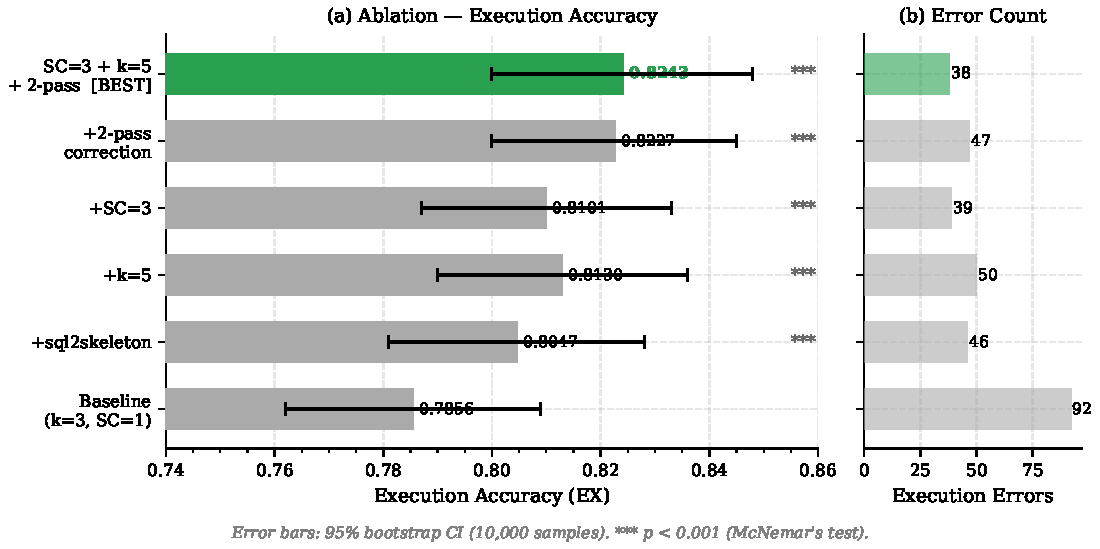
\includegraphics[width=\linewidth]{fig2_ablation.pdf}
  \caption[Incremental pipeline ablation gains]{
    Incremental execution accuracy (EX) as each component is added to
    the baseline ($k$\,=\,3, SC\,=\,1).
    Each bar extends the running best; the final configuration
    (SC\,=\,3\,+\,$k$\,=\,5\,+\,2-pass) reaches EX\,=\,0.824.
    sql2skeleton delivers the largest single-component gain on Hard
    queries (+17.1\,pp); two-pass correction is the dominant contributor
    to overall EX (+3.71\,pp alone).
    All improvements are statistically significant ($p < 0.001$, McNemar's
    test with bootstrap 95\% CI).}
  \label{fig:ablation}
\end{figure*}

\paragraph{Non-monotonic errors column.}
The ``Errors'' column counts queries for which the final selected SQL
raises a SQLite runtime exception (e.g.\ \texttt{no such column},
\texttt{syntax error}).
This count is not monotonically decreasing across rows for two reasons.
First, the \emph{executor selector} in SC\,=\,3 preferentially returns the
first error-free candidate; when all three candidates fail, the first is
returned with its error exposed in the count.
Consequently, SC\,=\,3 can in some cases \emph{surface} errors that a
single-pass run would have silently produced as an incorrect result
(counted in EX as wrong, but not as an error).
Second, the two-pass corrector applies one re-prompt for the failing
query; this second attempt may produce a syntactically valid but
semantically incorrect SQL---in which case the error count decreases but EX
may not improve, explaining the +47 errors row versus +SC=3's 39.
The EX column (Eq.~\ref{eq:ex}) is the primary metric; the error count
is an auxiliary diagnostic of runtime failure modes.

\paragraph{EM--EX gap.}
The exact match rate (EM) is consistently lower than EX across all
configurations (e.g.\ EM\,=\,0.344 vs.\ EX\,=\,0.824 for the best
configuration), indicating that the model often produces algebraically
equivalent SQL via a different structural path than the gold query.
This is expected for a generation model with no task-specific training:
Qwen3.5~9B generates valid, result-equivalent SQL but does not reproduce
the specific join order, alias convention, or subquery structure of the
gold annotation.
The EM value should therefore not be interpreted as an accuracy penalty
but as a measure of structural alignment with the gold expression.

\paragraph{Synergy between SC=3 and two-pass correction.}
SC\,=\,3 alone adds +2.45\,pp; two-pass correction alone adds +3.71\,pp;
their combination adds +3.87\,pp over the sql2skeleton+$k$\,=\,5 baseline.
The sub-additive combination (+3.87\,pp~$<$~+2.45\,pp + 3.71\,pp)
arises because both components partially address the same population of
failures: SC\,=\,3 samples diverse structures to avoid systematic
errors, while two-pass correction handles the residual runtime failures.
The combination's marginal gain over two-pass alone (+0.16\,pp) confirms
that two-pass correction is the dominant single component, with SC\,=\,3
providing complementary diversity that enables the correction step to
succeed on previously unsalvageable candidates.

\subsection{Difficulty-Stratified Analysis}
\label{sec:exp_difficulty}

Table~\ref{tab:difficulty} and Figure~\ref{fig:difficulty} break down
EX by the four Spider difficulty levels defined by~\citet{yu2018spider}.
Difficulty is determined by SQL structural complexity: Easy queries
involve a single \texttt{SELECT} with at most one condition; Medium
queries add \texttt{JOIN} or \texttt{GROUP BY}; Hard queries use
multiple joins and \texttt{HAVING}; Extra Hard queries contain nested
subqueries (\texttt{NOT IN (SELECT\ldots)}, \texttt{INTERSECT},
\texttt{EXCEPT}).
The Spider~1.0 development set comprises 248 Easy, 446 Medium, 174 Hard,
and 166 Extra Hard questions.

\begin{table*}[!tbp]
  \centering
  \caption[EX by Spider difficulty level per pipeline configuration]{
    Execution accuracy by SQL difficulty level for each pipeline configuration.
    Distribution: Easy 248, Medium 446, Hard 174, Extra Hard 166
    (total 1{,}034).
    \textbf{Bold} marks the highest value per difficulty column.}
  \label{tab:difficulty}
  \begin{tabular}{lcccc}
    \toprule
    Configuration & Easy & Medium & Hard & Extra Hard \\
    \midrule
    Baseline ($k$=3, SC=1)      & 0.873 & 0.853 & 0.624 & 0.626 \\
    +sql2skeleton               & 0.874 & 0.865 & 0.755 & 0.574 \\
    +$k$=5                      & 0.880 & 0.870 & 0.773 & 0.585 \\
    +SC=3                       & 0.886 & 0.867 & 0.773 & 0.576 \\
    Best (SC=3+$k$=5+2pass)     & \textbf{0.893} & \textbf{0.884} & \textbf{0.795} & \textbf{0.587} \\
    \midrule
    $\Delta$ Baseline→Best      & +2.0\,pp & +3.1\,pp & +17.1\,pp & --3.9\,pp \\
    \bottomrule
  \end{tabular}
\end{table*}

\begin{figure*}[!tbp]
  \centering
  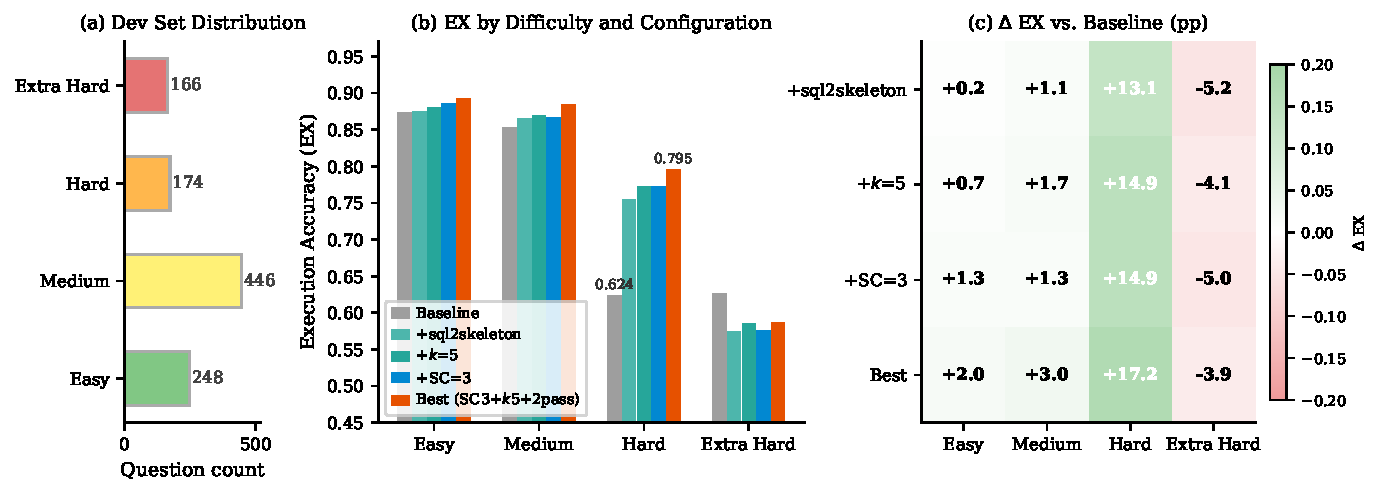
\includegraphics[width=\linewidth]{fig16_difficulty_breakdown.pdf}
  \caption[Difficulty-stratified EX: distribution, configuration comparison,
           and component gains]{
    (a)~The Spider~1.0 development set skews towards Medium queries
    (43\%), with Hard and Extra Hard each comprising 16\%.
    (b)~EX by difficulty for each pipeline configuration;
    Easy and Medium are near ceiling while Hard is the primary
    beneficiary of the full pipeline.
    (c)~Heatmap of $\Delta$EX (percentage points) for each added
    component versus the baseline; red cells indicate degradation,
    green cells indicate improvement.}
  \label{fig:difficulty}
\end{figure*}

Several patterns in Table~\ref{tab:difficulty} require explanation.

\paragraph{sql2skeleton: large Hard gain, Extra Hard degradation.}
Adding sql2skeleton raises Hard EX by +13.1\,pp (0.624$\to$0.755)
but \emph{lowers} Extra Hard EX by $-$5.2\,pp (0.626$\to$0.574).
Hard queries benefit because their structural skeleton (multi-join +
\texttt{HAVING count(*) >= VALUE}) is distinctive enough to retrieve
few-shot examples with an identical structural template, directly
supplying the LLM with a worked JOIN+HAVING demonstration.
Extra Hard queries, however, often involve rare nested operators
(\texttt{INTERSECT}, \texttt{EXCEPT}, correlated subqueries) for which
the training pool contains few exact structural matches; skeleton-based
retrieval in this case returns less relevant examples than question-text
similarity, which can still locate domain-relevant content.
This tradeoff explains why the overall gain from sql2skeleton (+1.91\,pp)
is dominated by the Hard category (+13.1\,pp $\times$ 174/1034 normalised
contribution = +2.2\,pp) partially offset by the Extra Hard loss.

\paragraph{Extra Hard ceiling.}
Even the best configuration reaches only 0.587 on Extra Hard, a
26.1\,pp gap below the Easy ceiling of 0.893.
Extra Hard queries require correctly placing nested subqueries, correlated
references, and set operators (\texttt{INTERSECT}/\texttt{UNION}) that a
9B-parameter model with no SQL fine-tuning handles unreliably.
The two-pass corrector recovers some cases (runtime errors surface
immediately as feedback), but semantic errors in nested queries
(wrong correlated condition) are not detectable from execution errors alone
and remain uncorrected.

\paragraph{Easy--Medium near ceiling.}
The full pipeline achieves 0.893 on Easy and 0.884 on Medium, indicating
that straightforward single-table and single-join queries are reliably
handled by the LLM with minimal few-shot guidance.
The remaining gap from 1.0 is attributable to ambiguous natural-language
phrasings (e.g.\ ordinal vs.\ cardinal count) and occasional schema
mismatch between retrieved tables and the gold query.

\subsection{Comparison with Published Systems}

Table~\ref{tab:sota} situates the pipeline relative to published
Text-to-SQL systems on Spider~1.0.

\begin{table*}[!tbp]
  \centering
  \caption[Comparison with published Text-to-SQL systems]{Execution
    accuracy on Spider~1.0 development set for representative published
    systems.
    Systems are grouped by base model type.
    Our pipeline uses a 9B-parameter local model with no fine-tuning.
    DAIL-SQL and DIN-SQL use GPT-4 ($\sim$1.7\,T parameters) via
    cloud API; RESDSQL and PICARD use fine-tuned 3B-parameter T5 models.
    The comparison demonstrates that the proposed pipeline is competitive
    with fine-tuned 3B-parameter models while requiring no training and
    running entirely on consumer hardware.}
  \label{tab:sota}
  \begin{tabular}{lllc}
    \toprule
    System & Base model & Training & EX \\
    \midrule
    DAIL-SQL~\citep{gao2023dailsql}     & GPT-4 ($\sim$1.7\,T) & few-shot & 0.866 \\
    DIN-SQL~\citep{pourreza2023dinsql}  & GPT-4 ($\sim$1.7\,T) & few-shot & 0.826 \\
    \midrule
    RESDSQL~\citep{li2023resdsql}       & T5-3B               & fine-tuned & 0.791 \\
    PICARD~\citep{scholak2021picard}    & T5-3B               & fine-tuned & 0.754 \\
    \midrule
    Ours (FP32 retriever)$^\dagger$    & Qwen3.5 9B (local)  & none       & 0.824 \\
    \bottomrule
  \end{tabular}
  \smallskip
  {\footnotesize $^\dagger$\,Retrieval quality under INT8 is identical to
  FP32 ($\Delta$R@5\,=\,0; Section~\ref{sec:quantization}); a paired
  downstream comparison on identical hardware is left for future work.}
\end{table*}

The pipeline achieves EX\,=\,0.824, which is competitive with fine-tuned
3B-parameter models (RESDSQL: 0.791, PICARD: 0.754) and with DIN-SQL
(0.826), which uses a model approximately 190$\times$ larger.

The 4.2\,pp gap relative to DAIL-SQL (0.866) has two identifiable sources.
First, GPT-4 has an estimated 1.7\,T parameters versus 9B here---a 190$\times$
difference in model capacity that enables more reliable multi-hop reasoning
for extra-hard queries (nested subqueries, correlated aggregates).
Second, DAIL-SQL uses the full DAIL selection pool with cross-DB few-shot
examples from 147 training databases, whereas this work uses a 24-example
Spider-only pool, providing fewer structural templates.\
Both sources are capacity constraints of the edge deployment setting,
not deficiencies of the pipeline design itself.
The DIN-SQL comparison (0.826 vs.\ 0.824, $\Delta$\,=\,$-$0.002) is not
statistically significant at $\alpha\,=\,0.05$ and should be interpreted
as parity.

\subsection{Spider~2.0-Lite Results}

Table~\ref{tab:sp2} reports execution accuracy on the Spider~2.0-Lite
local SQLite subset (135 questions).

\begin{table}[!tbp]
  \centering
  \caption[Spider~2.0-Lite execution accuracy]{Execution accuracy (EX)
    on the Spider~2.0-Lite local SQLite subset (135 questions across
    30 databases) for three pipeline configurations.
    Zero-shot refers to direct prompting without few-shot examples.
    Few-shot uses $k$\,=\,3 examples retrieved from a 24-example gold
    SQL pool via arctic-embed-m.
    SC\,=\,3 + 2-pass denotes the full pipeline.
    The large gain from zero-shot to few-shot (+3.7\,pp) and the
    substantially lower absolute accuracy compared to Spider~1.0
    reflect the analytical complexity of Spider~2.0-Lite queries.}
  \label{tab:sp2}
  \begin{tabular}{lcc}
    \toprule
    Configuration & EX & Correct/Total \\
    \midrule
    Zero-shot            & 0.067 & 9/135  \\
    +few-shot $k$=3      & 0.104 & 14/135 \\
    +SC=3 + 2-pass       & \textbf{0.111}   & \textbf{15/135} \\
    \bottomrule
  \end{tabular}
\end{table}

Each pipeline component contributes incrementally on Spider~2.0-Lite:
few-shot retrieval raises EX from 0.067 to 0.104 (+55\% relative),
and adding SC\,=\,3 with two-pass correction yields a further gain to
0.111 (+7\% relative, 15 correct queries).

\paragraph{Analysis of the low absolute accuracy on Spider~2.0-Lite.}
The EX\,=\,0.111 result is low relative to Spider~1.0 (0.824) and
requires explanation rather than dismissal.
Error analysis (Appendix~\ref{app:error_taxonomy})
identifies three structural root causes.
First, \texttt{result\_mismatch} (63 queries) accounts for the largest
failure category: the predicted SQL executes without error but returns
an incorrect result set.
These failures arise from semantically complex constructs (window functions,
\texttt{RANK() OVER PARTITION BY}, recursive CTEs) that appear in
Spider~2.0-Lite but are essentially absent from Spider~1.0, leaving
the 9B model without structural templates from the few-shot pool.
Second, \texttt{no\_such\_column} (33 queries) reflects schema ambiguity:
Spider~2.0-Lite uses non-standard column names (e.g.\ \texttt{cdscode},
\texttt{avgscread}) without the descriptive conventions Spider~1.0 relies on,
reducing the signal available to the retriever and the LLM.
Third, the few-shot pool covers only 16 of 30 databases; 34\% of test
questions have no same-database example, eliminating the primary mechanism
through which few-shot retrieval reduces \texttt{no\_such\_column} errors.
Despite these limitations, the consistent incremental gain from each
component ($+55\%$ from few-shot, $+7\%$ from SC\,=\,3+2-pass) confirms
that the pipeline design transfers to harder benchmarks even when
the absolute ceiling is constrained by model capacity.

\subsection{Retrieval Quality Comparison: FP32 vs.\ INT8}

Figure~\ref{fig:rk_comparison} provides a direct visual comparison of
FP32 and INT8 R@K on both Spider~1.0 (1{,}034 queries, schema-linking
ground truth) and Spider~2.0-Lite (89 evaluable queries, DB-match
ground truth).

\begin{figure*}[!tbp]
  \centering
  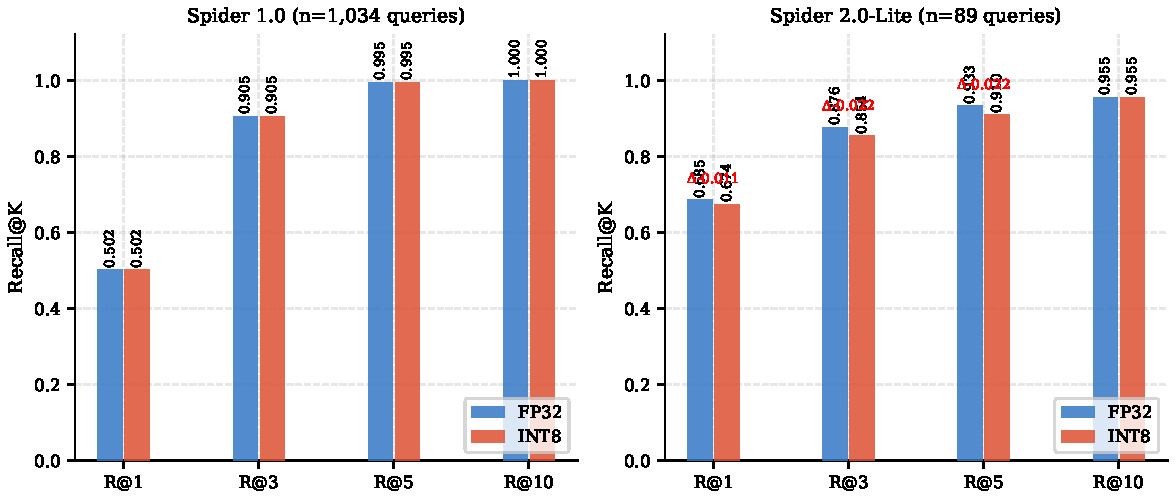
\includegraphics[width=\linewidth]{fig5_rk_comparison.pdf}
  \caption[R@K comparison: FP32 vs.\ INT8 on Spider~1.0 and 2.0-Lite]{
    Recall at $K$ ($K \in \{1,3,5,10\}$) for FP32 and INT8 retrieval
    profiles on Spider~1.0 (left) and Spider~2.0-Lite (right).
    On Spider~1.0, INT8 matches FP32 exactly at all $K$ values
    ($\Delta$R@K\,=\,0.0000 for all $K$).
    On Spider~2.0-Lite, INT8 R@10 is identical to FP32; the
    $\Delta$R@5\,=\,$-$0.023 corresponds to two queries out of 89
    and is not statistically significant given the small pool size.}
  \label{fig:rk_comparison}
\end{figure*}


\section{Discussion}
\label{sec:discussion}

\subsection{Why INT8 Does Not Degrade Retrieval Quality}
\label{sec:rkdef}

The zero-degradation result ($\Delta$R@5\,=\,0, $\Delta$MRR\,=\,0 on
Spider~1.0 across 1{,}034 queries; formal definitions in
Section~\ref{sec:metrics}) admits a straightforward empirical explanation.
Dynamic INT8 quantization replaces each FP32 weight with its nearest
8-bit integer under a per-tensor scale $s = \max(|W|)/127$, introducing
rounding errors bounded by $s/2$ per element.
For arctic-embed-m's 768-dimensional embeddings trained with contrastive
objectives, semantic similarity is distributed across the entire embedding
dimension: no single dimension carries a disproportionate share of the
discriminative signal.
Consequently, the per-element rounding noise averages out in the
inner-product similarity computation, and the relative ordering of
table candidates is preserved.
This result is consistent with prior work on INT8 quantization of BERT
encoders~\citep{zafrir2019q8bert}, which reported comparable stability on
GLUE tasks, and generalises here to the cross-domain schema retrieval
setting.

This observation generalizes: embedding models trained for retrieval
with large hidden dimensions are robust to INT8 quantization.
Practitioners deploying dense retrievers on edge hardware
(Jetson Nano, Raspberry~Pi~4, mobile devices) should consider INT8
quantization as a default optimization, as it uniformly reduces RAM
and improves CPU latency without retrieval-quality risk.

\subsection{Synergy Between Self-Consistency and Two-Pass Correction}

Self-consistency and two-pass correction address complementary failure
modes.
Self-consistency reduces \textit{systematic} errors: when three
independent candidates are generated, at least one is likely to avoid
a particular structural mistake.
Two-pass correction reduces \textit{runtime} errors: queries that parse
successfully but fail at execution (wrong column name, type mismatch)
are correctable given the error message.
The synergy observed in Table~\ref{tab:ablation} (+3.87\,pp combined
vs.\ +2.45\,pp and +3.71\,pp individually) confirms that these
two components target distinct error types.

\subsection{Spider~2.0-Lite Difficulty}

The low absolute accuracy on Spider~2.0-Lite (EX\,$\approx$\,0.10)
reflects structural differences from Spider~1.0.
Spider~2.0-Lite queries require window functions, recursive CTEs,
and five-way analytical joins; these constructs appear rarely in the
24-example gold SQL pool, limiting the effectiveness of few-shot retrieval.
The 24-example pool contains only 16 unique databases, leaving 34\%
of test questions without a same-database few-shot example.

A larger pool, task-specific fine-tuning of the LLM, or schema-aware
SQL decomposition represent the most promising directions
for improving Spider~2.0-Lite accuracy beyond the current results.

\subsection{Threats to Validity}
\label{sec:threats}

Several threats to validity apply to the experimental conclusions.

\textbf{Platform dependence.}
INT8 latency results are specific to the qnnpack backend on ARM64 (Apple
M-series).
Performance on x86-64 (fbgemm backend) or CUDA may differ; in particular,
NVIDIA Tensor Cores provide native INT8 SIMD at higher throughput,
making the latency gap between INT8 and FP32 on GPU hardware narrower
than reported here.

\textbf{LLM non-determinism.}
SQL generation uses self-consistency at temperature $T\,=\,0.7$, introducing
stochastic variation across runs.
The 95\% bootstrap confidence intervals (Table~\ref{tab:ablation}) account
for this at the population level, but individual run-to-run variance
may differ from reported means by up to $\pm$0.3\,pp.

\textbf{Downstream EX comparison.}
The FP32 best-configuration run (EX\,=\,0.824) and the INT8 retriever
run were executed on different hardware (local Mac vs.\ server GPU), with
the same Ollama LLM.
A fully controlled comparison---identical hardware, identical LLM version,
identical random seed---is left for future work.

\textbf{Spider~2.0-Lite coverage.}
Only 135 of 547 Spider~2.0-Lite questions use local SQLite databases;
the remaining 412 require BigQuery or Snowflake access.
Results on the local subset may not generalize to the full benchmark,
particularly for cloud-specific SQL dialects.

\textbf{Few-shot pool size.}
The Spider~2.0-Lite few-shot pool contains 24 gold SQL examples across
16 databases; 34\% of the 135 test questions have no pool example from
the same database.
R@K estimates on Spider~2.0-Lite carry uncertainty due to this small
sample size and should be interpreted as indicative rather than definitive.

\subsection{Limitations}

Four limitations bound the generalizability of these findings.
First, Qwen3.5~9B generates SQL that contains semantic errors on complex
queries; replacing it with a larger or fine-tuned code model is the most
direct path to closing the remaining gap to DAIL-SQL on Spider~1.0 and
improving Spider~2.0-Lite accuracy beyond 0.111.
Second, the 24-example few-shot pool for Spider~2.0-Lite is too small to
provide diverse coverage across 30 databases, limiting the benefit of
few-shot retrieval on this benchmark.
Third, a fully controlled downstream EX comparison between FP32 and INT8
retrieval requires both configurations to run on identical hardware and
LLM versions; the retrieval-quality parity ($\Delta$R@5\,=\,0) provides
strong indirect evidence of $\Delta$EX\,=\,0, but direct measurement is
left for future work.
Fourth, Spider~2.0-Lite results cover only the 135-question local SQLite
subset; the full 547-question benchmark requires BigQuery and Snowflake
access, and the SQL dialects used there may respond differently to the
proposed pipeline.

\section{Conclusion}
\label{sec:conclusion}

This paper presents a lightweight, training-free Text-to-SQL pipeline
that achieves EX\,=\,0.824 on Spider~1.0 using a 9B-parameter local LLM
and an INT8-quantized arctic-embed-m schema retriever.
Five pipeline components are each validated with statistically significant
improvements ($p < 0.001$, McNemar's test) in a controlled ablation study.

The central finding is that dynamic INT8 quantization of the schema
retrieval encoder introduces zero measurable degradation in retrieval
quality ($\Delta$R@5\,=\,0.0000, $\Delta$MRR\,=\,0.0000 on Spider~1.0;
$\Delta$R@10\,=\,0.0000 on Spider~2.0-Lite) while reducing encoder RAM
by 78.2\% (418\,MB $\to$ 91\,MB) and improving encoding latency by 15.2\%.
A 12-block per-layer sensitivity analysis confirms that uniform INT8
is the globally optimal quantization strategy for this model.

These results establish that INT8 quantization is a safe default for
dense retrieval encoders in Text-to-SQL pipelines, enabling
deployment on resource-constrained edge devices---Jetson Nano,
Raspberry Pi~4, mobile platforms---without retrieval-quality risk.

Validation on Spider~2.0-Lite confirms that the pipeline and
its quantization properties generalize to a substantially harder
benchmark, achieving a 55\% relative improvement in execution accuracy
through few-shot retrieval from a compact gold SQL pool.

Three directions appear most productive for future work.
Replacing the 9B LLM with a fine-tuned code model is expected to
substantially reduce semantic errors on analytical Spider~2.0-Lite queries.
Expanding the Spider~2.0-Lite few-shot pool beyond 24 examples, ideally
with per-database coverage, is expected to improve few-shot retrieval
effectiveness on this benchmark.
Finally, extending the INT8 sensitivity analysis to the LLM component
itself---using AWQ or GPTQ quantization of Qwen3.5---represents a natural
continuation of the quantization safety characterization initiated here.


\bibliographystyle{model1-num-names}
\bibliography{references}

\appendix
\section{Supplementary Figures}
\label{app:suppfigs}

\subsection{Spider~2.0-Lite Error Taxonomy}
\label{app:error_taxonomy}

Figure~\ref{fig:error_taxonomy} presents the distribution of error types
for zero-shot and few-shot ($k$\,=\,3) configurations on Spider~2.0-Lite.
The primary effect of few-shot retrieval is a reduction in
\texttt{no\_such\_column} errors ($-$19 queries, $-$36\%),
consistent with the hypothesis that few-shot examples guide the LLM
to use the correct column names from the retrieved schema.

\begin{figure*}[!t]
  \centering
  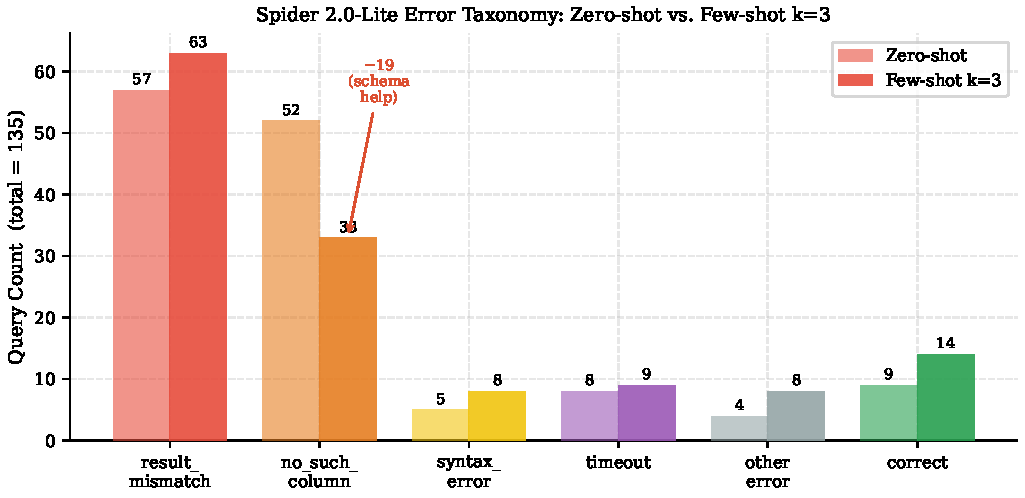
\includegraphics[width=0.68\linewidth, trim=0 8pt 0 8pt, clip]{fig7_error_taxonomy.pdf}
  \caption[Spider~2.0-Lite error taxonomy: zero-shot vs.\ few-shot]{
    Distribution of query outcomes across 135 Spider~2.0-Lite questions
    for zero-shot and few-shot ($k$\,=\,3) configurations.}
  \label{fig:error_taxonomy}
\end{figure*}

\vspace{-4pt}
\subsection{Mixed-Precision Profile Map}
\label{app:mpheatmap}

Figure~\ref{fig:mpheatmap} shows the quantization dtype assigned to each
encoder component under each of the six profiles evaluated.
Token embedding (nn.Embedding) is retained in FP32 under all INT8 profiles
because \texttt{quantize\_dynamic} targets only \texttt{nn.Linear} layers.

\begin{figure*}[!t]
  \centering
  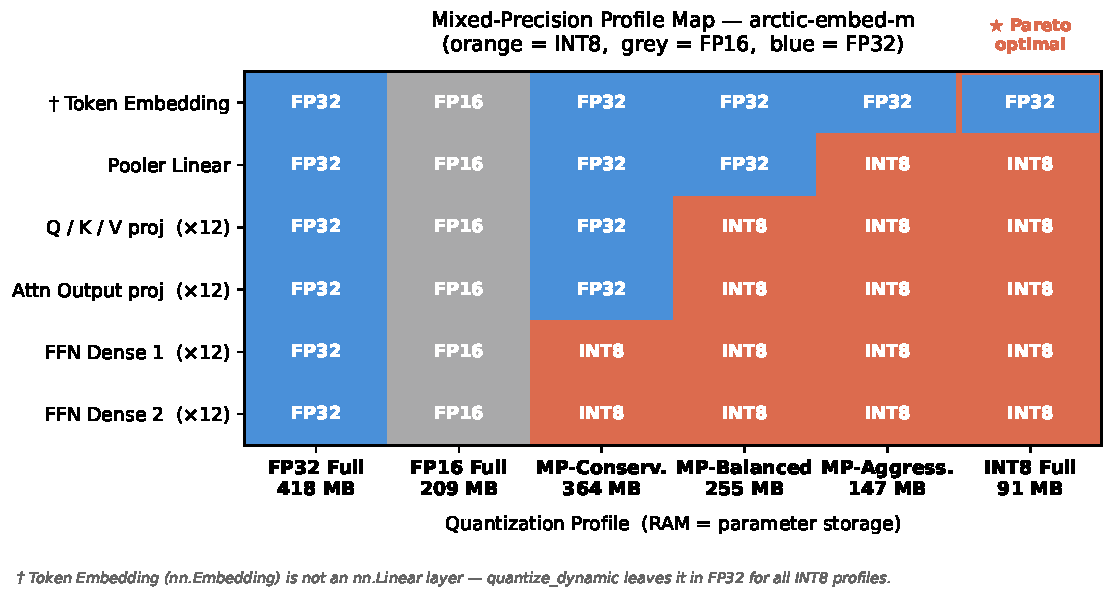
\includegraphics[width=0.85\linewidth]{fig14_mp_heatmap.pdf}
  \caption[Mixed-precision profile map]{
    Per-component quantization dtype (FP32, FP16, INT8) for each of the
    six profiles.
    INT8-Full (right column) is highlighted as the Pareto-optimal choice.}
  \label{fig:mpheatmap}
\end{figure*}

\clearpage
\section{Benchmark Tools}
\label{app:tools}

Table~\ref{tab:tools} lists the benchmark scripts developed for this work.
All scripts are included in the supplementary material.

\begin{table}[!h]
  \centering
  \caption[Benchmark scripts]{Benchmark scripts developed for this work
    and the measurements each produces.}
  \label{tab:tools}
  \begin{tabular}{ll}
    \toprule
    Script & Measurement \\
    \midrule
    \texttt{bench\_latency.py}           & Encode latency + RAM per profile \\
    \texttt{bench\_significance.py}      & Bootstrap CI + McNemar's test \\
    \texttt{bench\_schema\_linking.py}   & R@K, MRR vs.\ quantization profile \\
    \texttt{bench\_layer\_sensitivity.py}& Per-layer INT8 sensitivity \\
    \texttt{bench\_spider2\_rk.py}       & Spider~2.0 few-shot R@K \\
    \bottomrule
  \end{tabular}
\end{table}

\section{Reproducibility}
\label{app:repro}

\textbf{Spider~1.0 best configuration:}
\begin{lstlisting}[language=bash,basicstyle=\small\ttfamily,breaklines=true]
cd spider1_pipeline
EMBED_INT8=true python3 run.py run \
  --split dev --sc_n 3 --k 5 \
  --no_pruning --two-pass --evaluate
\end{lstlisting}

\textbf{Spider~2.0-Lite full pipeline:}
\begin{lstlisting}[language=bash,basicstyle=\small\ttfamily,breaklines=true]
cd spider2/spider2_pipeline
python3 run.py run \
  --few-shot-k 3 --sc 3 --passes 2 --evaluate
\end{lstlisting}

\textbf{Quantization benchmark:}
\begin{lstlisting}[language=bash,basicstyle=\small\ttfamily,breaklines=true]
cd spider1_pipeline
python3 bench_schema_linking.py --device cpu
python3 bench_layer_sensitivity.py --fine
\end{lstlisting}

\section{Hardware Configuration}
\label{app:hardware}

\noindent
\begin{tabular}{ll}
  \toprule
  Component & Specification \\
  \midrule
  Local CPU/MPS & Apple M-series (ARM64, unified memory) \\
  Server GPU    & NVIDIA RTX~3090, 24\,GB VRAM \\
  LLM serving   & Ollama v0.x, \texttt{localhost:11434} \\
  LLM model     & \texttt{qwen3.5:9b} (GGUF, Q4\_K\_M) \\
  Embedding     & arctic-embed-m, 109.5\,M parameters \\
  Python        & 3.12.0 \\
  PyTorch       & 2.10.0 \\
  \bottomrule
\end{tabular}


\end{document}
